\section{Designing the graphical user interface}
To familiarize ourselves with the context of our application, the team did a lot of research in the beginning of the project, as described in chapter~\ref{sec:prestudy}. A part of that process was to find already existing solutions and hopefully get some ideas about what functionality that might be useful in our application, but also regarding the graphical user interface design.

This section summarizes the team's process of designing the graphical user interface for the app.

\subsection{Branding}
An important part of the design process was to make sure the app was both user friendly and well customized for its purpose. As it did not really exist a pack of icons that suited all of our needs, the team created custom icons for the different tabs and devices so that the functions within each tab would become more clear for the user.

The team also decided to change the name of the app, originally named ''UbiSolar''.\todo[inline]{We came to the conclusion that, considering that the purpose of the app was to increase the awareness of power consumption, the app should have a name that reflected this purpose. Hence, we had a brainstorming session, which lead to the name ''Wattitude'', a composition of watt and attitude (towards power consumption), an idea that was well received by the customer.}



\subsection{Prototyping}
On our first meeting with the customer, the customer requested that the team should figure out what functionality that might be in the app. To achieve this, the team had a brainstorming session, which resulted in a paper-mockup of the app. An example of this early prototype is shown in figure~\ref{fig:protoa}. This prototype laid the foundation on our further development and was of big help when specifying both the functional and non-functional requirements.

\begin{figure}[H]
  \centering
  \subbottom[\label{fig:protoa}Paper-prototype of a list of devices where a power producing device is selected.]{%
\includegraphics[width=0.3\textwidth]{ch/devProcess/fig/paperprototype.png}}
\quad
  \subbottom[\label{fig:protob} Digitalized prototype of list of devices on proto.io]{%
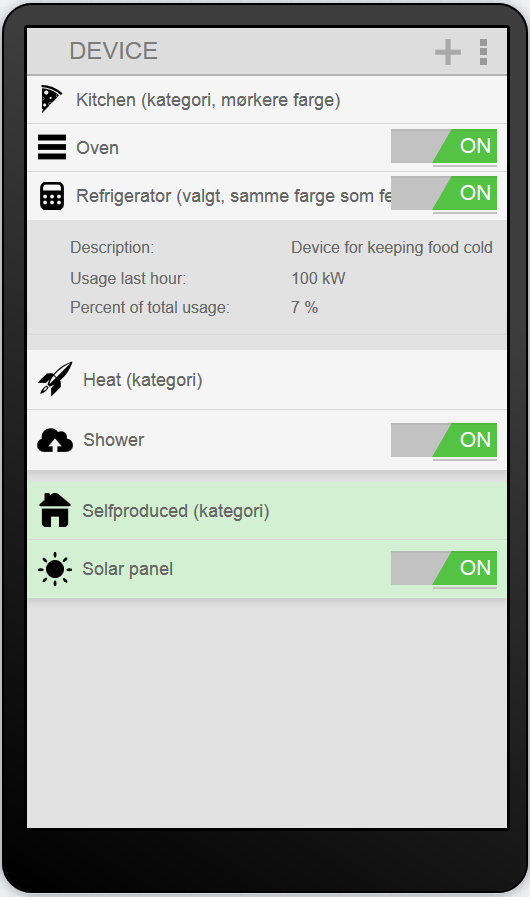
\includegraphics[width=0.3\textwidth]{ch/devProcess/fig/device.png}}
\quad
  \subbottom[\label{fig:protoc} Screenshot of list of devices in app]{%
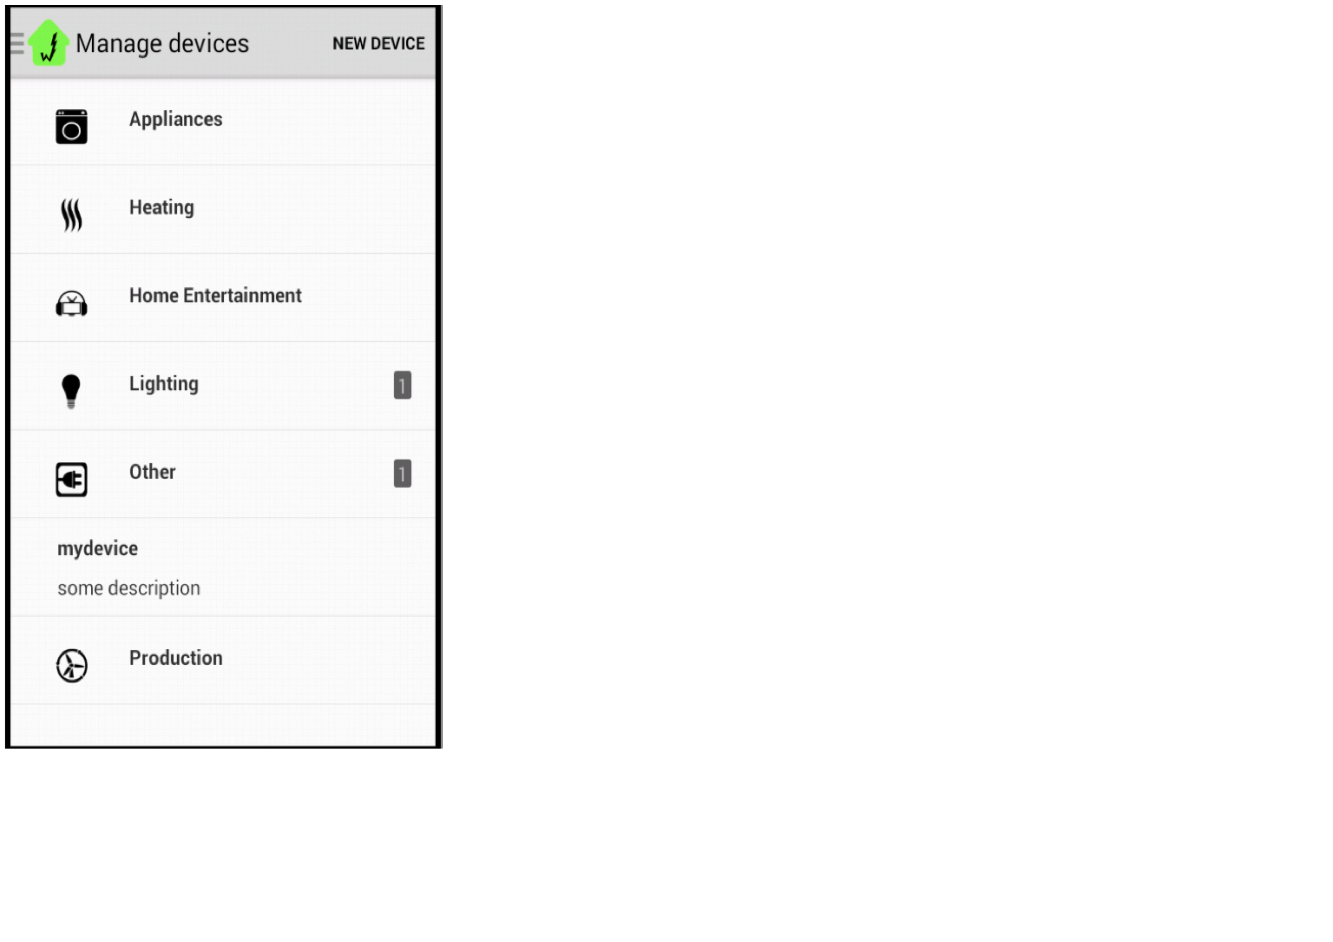
\includegraphics[width=0.3\textwidth]{ch/devProcess/fig/app.png}}
\caption{The evaluation: From prototype to product}
\end{figure}

\noindent However, a paper-prototype also may have some drawbacks, as suggested by Snyder~\cite{paperprototype}. For instance, it is hard to incorporate changes without having to re-do a lot of the work that has already been done. It is also very static, and does not give the right impression on how the actual end product might look like. Therefore, the team moved on to a more digitalized solution, namely the web page proto.io~\cite{protoio}, where it was easier to show how the layout states changed when an action was performed. An example screenshot of this prototype is shown in figure~\ref{fig:protob}.

After the prototyping was done, the team was ready to move on to implementing the app in Android. An example screenshot of the finalized app is displayed in figure~\ref{fig:protoc}.

